\documentclass[a4paper]{article}

\usepackage[utf8]{inputenc}
\usepackage[european, siunitx]{circuitikz}
\usepackage{mathtools}
\usepackage{float}
\usepackage{hyperref}

\author{Nao Pross}
\title{Tastiera Sonora con Arduino}

\inputencoding{utf8}

\begin{document}
	\maketitle
	
	% Elettronica
	\section{Elettronica}
		Il circuito é costituito da 5 bottoni e uno speaker. Per questioni di spazio non é stato
		possibile utilizzare un bottone per ogni nota della scala, quindi ci sono 4 bottoni per
		suonare e uno per cambiare dalla prima parte, alla seconda della scala (verrà spiegato
		meglio nella sezione software). Tutti i componenti sono alimentati a \SI{5}{\volt} forniti
		da Arduino.\\\\
		Nota: lo schema é stato ridotto, quindi le maglie $S_{eb}$ e $S_{fc}$
		sono state rappresentate in un unica indicata con $S_{nn}$ poiché sono identiche alle altre.
		
		\begin{figure}[h] \centering \begin{circuitikz}
					% Power
			\draw	(0, 1)		to[voltage source, v=$\SI{5}{\volt}$]		(0, -1)
					(0, 1)		to[short]										(0, 2)
					(0, 2)		to[short]										(2, 2)
					(0, -2)		node[rground]{}								(0, -3)
					% S c4
					(2, 2)		to[push button, l=$S_{cg}$, -*]				(2, 0)
					(2, 0)		node[right=.5em]{$Pin_2$}					(2, 0)
					(2, 0)		to[R=4.7<\kilo\ohm>]							(2, -2)
					(2, -2)		to[short]										(0, -2)
					(0, -2)		to[short]										(0, -1)
					% S d4
					(2, 2)		to[short]										(4, 2)
					(4, 2)		to[push button, l=$S_{da}$, -*]				(4, 0)
					(4, 0)		node[right=.5em]{$Pin_3$}						(4, 0)
					(4, 0)		to[R=4.7<\kilo\ohm>]							(4, -2)
					(4, -2)		to[short]										(2, -2);
					% S e4 ... S b4
			\draw[dotted]
					(6, 2)		to[push button, l=$S_{nn}$, -*]				(6, 0)
					(6, 0)		node[right=.5em]{$Pin_n$}					(6, 0)
					(6, 0)		to[R=4.7<\kilo\ohm>]							(6, -2);
					% S shift
			\draw	(4, 2)		to[short]										(8, 2)
					(8, 2)		to[push button, l=$S_s$, -*]					(8, 0)
					(8, 0)		node[right=.5em]{$Pin_6$}					(8, 0)
					(8, 0)		to[R=4.7<\kilo\ohm>]							(8, -2)
					(8, -2)		to[short]										(4, -2)
					% Speaker
					(10, 2)		node[above=.5em]{$Pin_7$}					(10, 2)
					(10, 2)		to[short, o-]										(10, 1)
					(10, 1)		to[ageneric, l=Speaker]						(10, -1)
					(10, -1)	to[short]										(10, -2)
					(10, -2)	to[short]										(8, -2);				
		\end{circuitikz}
		\caption{Circuito Elettronico}
		\end{figure}
		
	\section{Software}
		\subsection{Lettura dello stato della tastiera}
			Le note musicali riprodotte sono una scala, da $C4$ a $C5$, quindi 8.
			Purtroppo non essendoci spazio sufficiente per attaccare 8 bottoni si é dovuto
			utilizzare 4 bottoni da tastiera e uno da Shift.
			
			\begin{table}[H]
				\centering \begin{tabular}{ | l l l l l l l l | }
				\hline
				Do & Re & Mi & Fa & Sol & La & Si & Do \\
				C4 & D4 & E4 & F4 & G4 & A4 & B4 & C5	\\
				\hline
				\end{tabular}
				\caption{Note in notazione a lettere rispetto alla notazione da solfeggio.}
			\end{table}
			
			Il bottone Shift, rappresentato come $S_s$ nella Figura 1 modifica il comportamento
			degli altri 4 bottoni nel seguente modo:
			``Se premuto quando $S_s$ é spento un bottone fa emettere una nota tra $C4$ e $F4$,
			quindi tra le prime 4 della scala. Altrimenti viene emessa una nota tra $G4$ e $C5$,
			le ultime 4 della scala.''
			
			\begin{table}[h]
				\begin{center} \begin{tabular}{ | l | r r | }
					\hline
					$S_{nn}$		&		$S_s = 0$	&	$S_s = 1$ \\
					\hline
					$S_{cg}$	&	$C4$	&	$G4$	\\
					$S_{da}$	&	$D4$	&	$A4$	\\
					$S_{eb}$	&	$E4$	&	$B4$	\\
					$S_{fc}$	&	$F4$	&	$C5$	\\
					\hline
				\end{tabular} \end{center}
				\caption{Tabella che mostra come $S_s$ modifica l'emissione del suono.}
			\end{table}

		\subsection{Frequenze}
			Lo speaker viene alimentato da una tensione a onda quadra di duty cycle 50\% fornita
			dal $Pin_7$, la frequenza di quest'ultima viene controllata da una funzione integrata in Arduino
			\texttt{tone(int pin, unsigned int frequency)}.\\\\
			Le frequenze utilizzate per produrre le note sono prese da \\
			\url{http://www.seventhstring.com/resources/notefrequencies.html}
			
			\begin{table}[h]
				\begin{center} \begin{tabular}{ | c l | c | }
					\hline
					Nota  & & Frequenza \\
					\hline
					$C4$ & Do & \SI{262}{\hertz} \\
					$D4$ & Re & \SI{294}{\hertz} \\
					$E4$ & Mi & \SI{330}{\hertz} \\
					$F4$ & Fa & \SI{349}{\hertz} \\
					$G4$ & Sol & \SI{392}{\hertz} \\
					$A4$ & La & \SI{440}{\hertz} \\
					$B4$ & Si & \SI{494}{\hertz} \\
					$C5$ & Do & \SI{523}{\hertz} \\
					\hline
				\end{tabular} \end{center}
				\caption{Frequenze delle note musicali.}
			\end{table}
		
		\subsection{Codice Sorgente}
			Il codice sorgente in \texttt{C++} si trova sul mio GitHub in un repository
			chiamato \texttt{2samb\_hw\_and\_sw} nella cartella \texttt{\_01\_keyboard} o più semplicemente
			al seguente link: \\
			\url{https://github.com/NaoPross/samb2_hw_and_sw/tree/master/_01_keyboard}s

		\subsection{Struttogramma}
			\begin{figure}[h!] \centering
				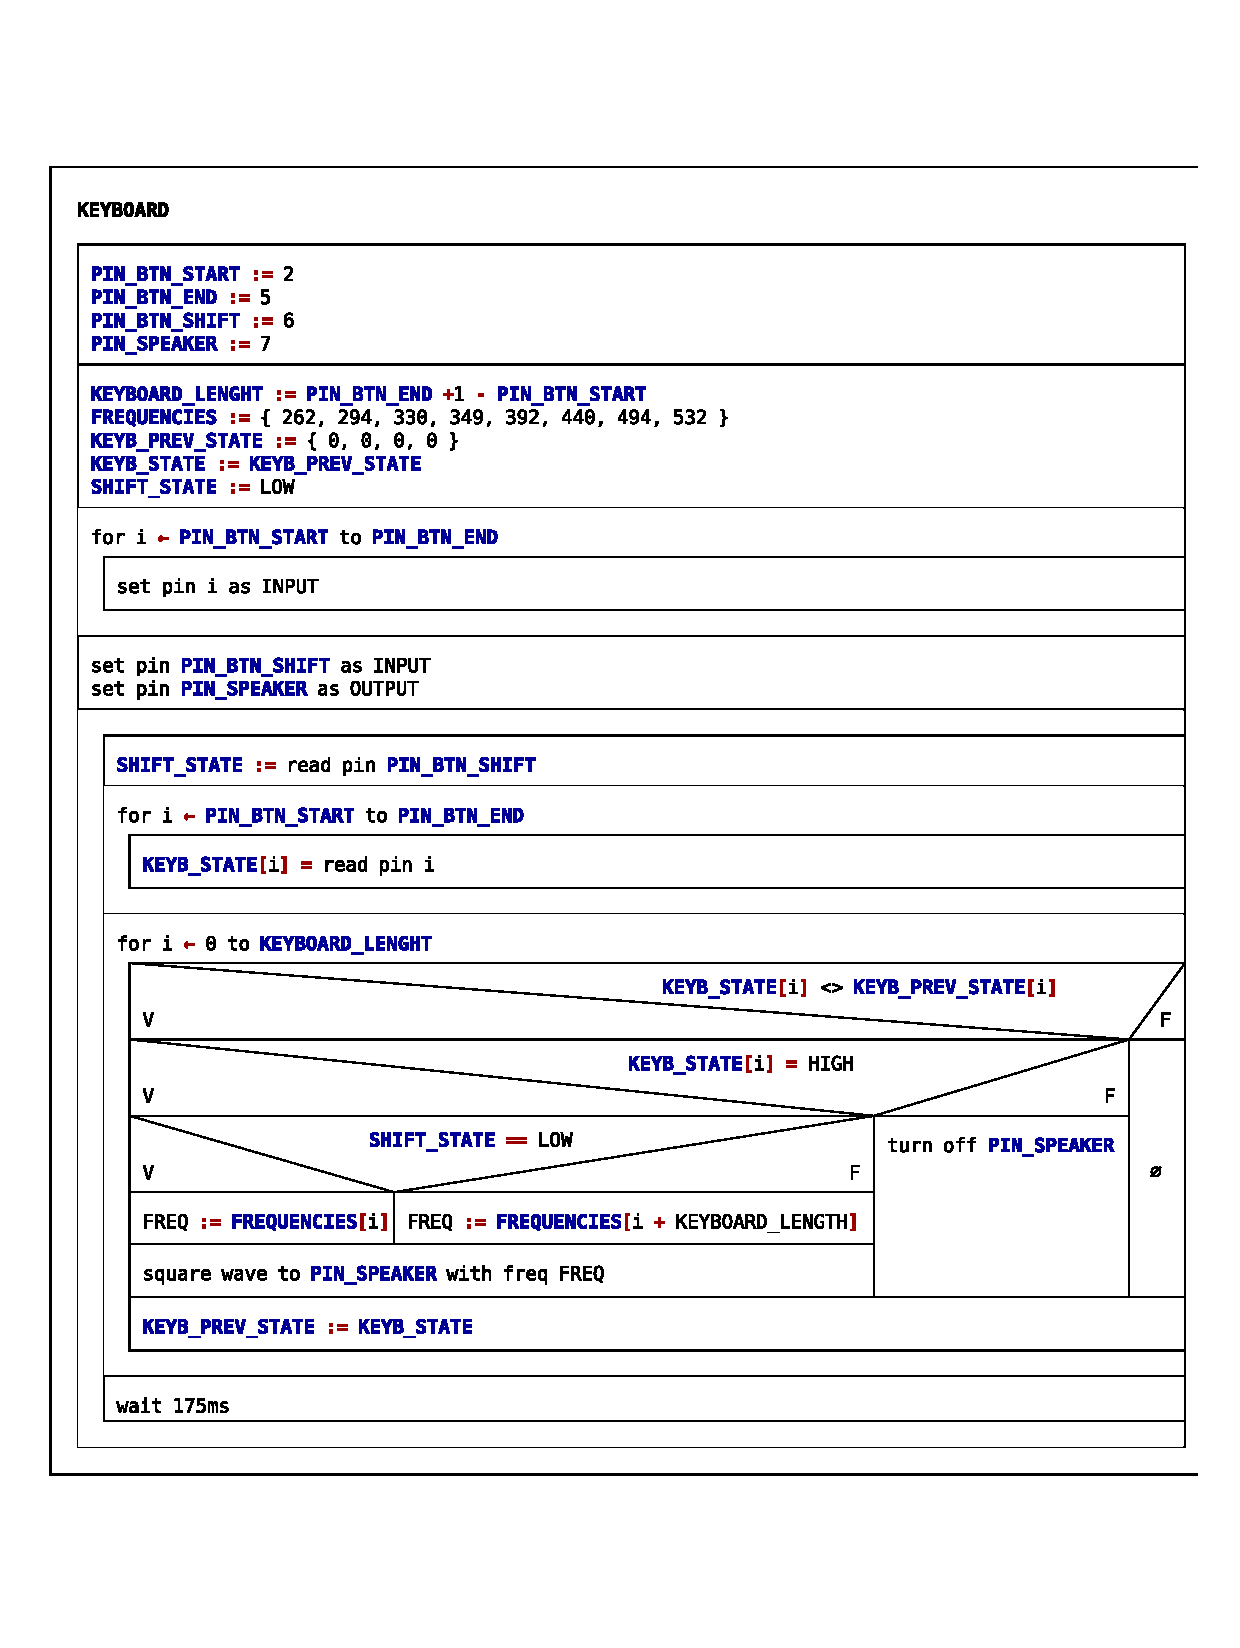
\includegraphics[keepaspectratio=true, width=45em, trim=10em 5em 0 20em]{KEYBOARD.pdf}
				\caption{Diagramma Nassi-Schneidermann del programma}
			\end{figure}
			
\end{document}